\subsection{Judas}

For this project, we will be working with data recorded from BANE-NOR, where a train is travelling between Trondheim and Storen the 31st of august 2021 \footnote{Working with national infrastructure requires security clearance, see \ref{app:conf} for more details}. Data is split between 5000 sensor channels, lasting us a day.
The data is recorded in \acrshort{hdf5} files, with each file containing 20000 samples for 10 seconds, giving us a sample rate of $2000Hz$. The


\begin{table}[h]
\centering
\begin{tabular}{|r|r|r|r|r|}
\hline
\textbf{1}                & \textbf{2}               & \multicolumn{1}{c|}{\textbf{...}} & \textbf{n-1}             & \textbf{n}               \\ \hline
1f-3                      & 2.3f-5                   & 4f-4                              & 3.4f-6                   & 3f-1                     \\ \hline
3f-1                      & 3f-1                     & 3f-1                              & 3f-1                     & 3f-1                     \\ \hline
\multicolumn{1}{|c|}{...} & \multicolumn{1}{c|}{...} & \multicolumn{1}{c|}{...}          & \multicolumn{1}{c|}{...} & \multicolumn{1}{c|}{...} \\ \hline
4f-2                      & 3f-1                     & 3f-1                              & 3f-1                     & 3f-1                     \\ \hline
\end{tabular}
\caption{Table explaining how the table looks like}
\label{fig:datatable}
\end{table}



\begin{figure}[h]
    \centering
    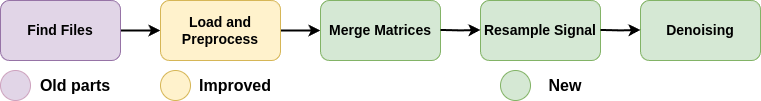
\includegraphics{figures/dataflow.png}
    \caption{Dataflow from we read HDF5 files to we are ready to train}
    \label{fig:dataflow}
\end{figure}

\subsection{Pre processing}

\subsubsection{Resampling and Channel decimation}

Following our previous work \cite{projthesis}, the following improvements have been made to \texttt{Judas}: 

\begin{enumerate}
    \item Judas now make use of multiple processors contra multithreading, seeing major speedups.
    \item Function \texttt{load\_DAS\_files} now writes processed data to a single file back.
    \item Methods for resampling and chann
\end{enumerate}


\subsubsection{Window and Filter operations}

After the data has been loaded \cite{projthesis}, it's still not ready for processing. 

The function \lstinline|process_DAS_data| takes in the signal data, perform a tukey \ref{dsp:tukey} window algorithm over it. We then run a band-pass filter algorithm with Butterworth over it to extract the and 

\begin{figure}[h]
    \centering
    \lstinputlisting[language=Julia]{code/procdasdata.jl}
    \caption{Process DAS data function}
    \label{fig:procdasdata}
\end{figure}


After applying a window function and a filter function to combat oscilleration, we're now ready to run an fft over this data. 


The 

\begin{figure}[h]
    \centering
    \includegraphics{figures/banenor_20210831.png}
    \caption{Heatmap of the processed train data during the 31st of august 2021 from Trondheim to Storen}
    \label{fig:trdstrdas}
\end{figure}

\subsection{Data preparation before Training} 

After the preprocessing, some final work must be done before we can train the model. Normalization, also called data standardization, 
is a basic staple of preprocessing, we  . This normalization makes sure all the values . For our model, we use z-score normalization, 
which normalizes vales to be in the range 0 to 1. The f

\begin{equation}
    x' = \frac{x - \mu}{x}
\end{equation}

This method is implemented as such in \texttt{Flux.jl}

\begin{figure}[h]
    \centering
    \lstinputlisting[language=Julia]{code/norm.jl}
    \caption{Flux normalization function}
    \label{fig:normalize_data}
\end{figure}

Where $\mu$ is the mean of the data, and $\sigma$ is the standard deviation of data.

\subsubsection{Data augmentation}